\documentclass[a0paper,portrait]{baposter}
\usepackage{wrapfig}
\usepackage{lmodern}
\usepackage[utf8]{inputenc} %unicode support
\usepackage[T1]{fontenc}
\selectcolormodel{cmyk}
\graphicspath{{figures/}} % Directory in which figures are stored
\usepackage{hyperref}
\newcommand{\compresslist}{\setlength{\itemsep}{0pt}\setlength{\parskip}{1pt}\setlength{\parsep}{0pt}}
\newenvironment{boenumerate}{\begin{enumerate}\renewcommand\labelenumi{\textbf\theenumi.}}{\end{enumerate}}

\begin{document}
	\definecolor{darkgreen}{cmyk}{0.8,0,0.8,0.45}
	\definecolor{lightgreen}{cmyk}{0.8,0,0.8,0.25}
	\begin{poster}
		{
			grid=false,
			headerborder=open, % Adds a border around the header of content boxes
			colspacing=1em, % Column spacing
			bgColorOne=white, % Background color for the gradient on the left side of the poster
			bgColorTwo=white, % Background color for the gradient on the right side of the poster
			borderColor=darkgreen, % Border color
			headerColorOne=lightgreen, % Background color for the header in the content boxes (left side)
			headerColorTwo=lightgreen, % Background color for the header in the content boxes (right side)
			headerFontColor=white, % Text color for the header text in the content boxes
			boxColorOne=white, % Background color of the content boxes
			textborder=rounded, %rectangle, % Format of the border around content boxes, can be: none, bars, coils, triangles, rectangle, rounded, roundedsmall, roundedright or faded
			eyecatcher=false, % Set to false for ignoring the left logo in the title and move the title left
			headerheight=0.11\textheight, % Height of the header
			headershape=rounded, % Specify the rounded corner in the content box headers, can be: rectangle, small-rounded, roundedright, roundedleft or rounded
			headershade=plain,
			headerfont=\Large\textsf, % Large, bold and sans serif font in the headers of content boxes
			%textfont={\setlength{\parindent}{1.5em}}, % Uncomment for paragraph indentation
			linewidth=2pt % Width of the border lines around content boxes
		}
		{}
		{
			{\small Projet de Fin d'Études 2022-2023}
			\sf\vspace{0.3em}\\
			\\\textsf
			{Navigation et contrôle multi-robots pour l'inspection acoustique de structures métallique}
		}
		{
			\sf\vspace{0.5em}\\
			Brandon ALVES
			\vspace{0.1em}\\
			\small{
				Département Informatique, INSA Lyon - CITI Lab. INSA - INRIA
				\vspace{0.2em}\\
				bdasilvaal@insa-lyon.fr
				\vspace{0.2em}\\
			}
		}
		{
			\hspace{0.5cm}
			
\includegraphics[height=1cm]{graphics/LogoStructureAccueil.png}
			\hspace{0.5cm}
			
\includegraphics[height=1cm]{graphics/insa}
		}
		\headerbox{1. Introduction}{name=introduction,column=0,row=0,span=3}{
			Saepissime igitur mihi de amicitia cogitanti maxime illud considerandum videri solet, utrum propter imbecillitatem atque inopiam desiderata sit amicitia, ut dandis recipiendisque meritis quod quisque minus per se ipse posset, id acciperet ab alio vicissimque redderet, an esset hoc quidem proprium amicitiae, sed antiquior et pulchrior et magis a natura ipsa profecta alia causa. Amor enim, ex quo amicitia nominata est, princeps est ad benevolentiam coniungendam. Nam utilitates quidem etiam ab iis percipiuntur saepe qui simulatione amicitiae coluntur et observantur temporis causa, in amicitia autem nihil fictum est, nihil simulatum et, quidquid est, id est verum et voluntarium.
		}
		\headerbox{2. Problématique}{name=model,column=0,below=introduction,span=1}{
			Iis igitur est difficilius satis facere, qui se Latina scripta dicunt contemnere. in quibus hoc primum est in quo admirer, cur in gravissimis rebus non delectet eos sermo patrius, cum idem fabellas Latinas ad verbum e Graecis expressas non inviti legant. quis enim tam inimicus paene nomini Romano est, qui Ennii Medeam aut Antiopam Pacuvii spernat aut reiciat, quod se isdem Euripidis fabulis delectari dicat, Latinas litteras oderit?

			\begin{center}
				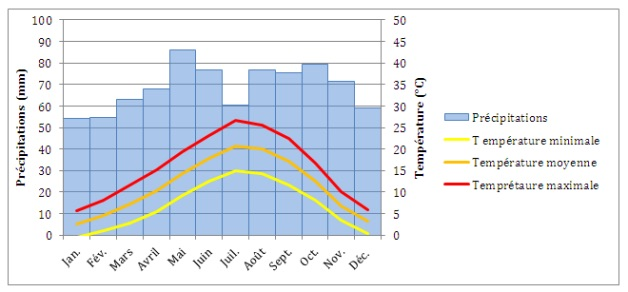
\includegraphics[width=\linewidth]{graphics/DiagrammeThil.jpg}
			\end{center}
		}
		\headerbox{3. La méthode des moments}{name=mcs,column=0,below=model,span=1}{
			La méthode des moments est un outil d'estimation intuitif qui date du début des statistiques.

			\textit{Elle consiste à estimer les paramètres recherchés en égalisant certains moments théoriques (qui dépendent de ces paramètres) avec leurs contreparties empiriques. L'égalisation se justifie par la loi des grands nombres qui implique que l'on peut "approcher" une espérance mathématique par une moyenne empirique. On est donc amené à résoudre un système d'équations.}
			\\\hfill \url{https://fr.wikipedia.org/wiki/Méthode_des_moments_(statistiques)}~\cite{DBLP:journals/eor/LayerJSF20}.

			\begin{center}
				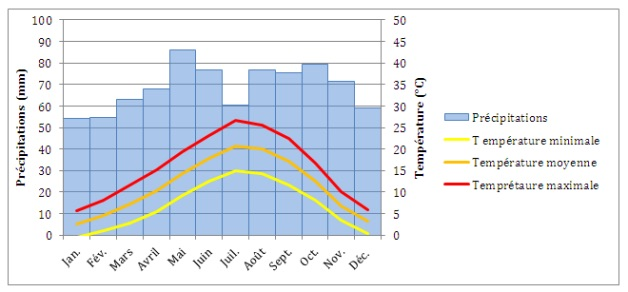
\includegraphics[width=\linewidth]{graphics/DiagrammeThil.jpg}
			\end{center}
		}
		\headerbox{4. Proposition de solution}{name=screen,span=2,column=1,below=introduction}{
			Dumque ibi \textbf{diu moratur commeatus opperiens, quorum translationem} ex Aquitania verni imbres solito crebriores prohibebant auctique torrentes, Herculanus advenit protector domesticus, Hermogenis ex magistro equitum filius, apud Constantinopolim, ut supra rettulimus, populari quondam turbela discerpti. quo verissime referente quae Gallus egerat, damnis super praeteritis maerens et futurorum timore suspensus angorem animi quam diu potuit emendabat.

			\begin{center}
				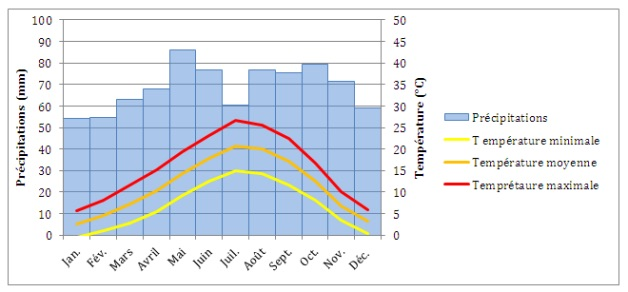
\includegraphics[width=0.85\linewidth]{graphics/DiagrammeThil.jpg}
			\end{center}
		}
		\headerbox{5. Évaluation de la proposition}{name=sea,span=2,column=1,below=screen}{
			\begin{wrapfigure}{l}{0.3\textwidth}
				\begin{center}
					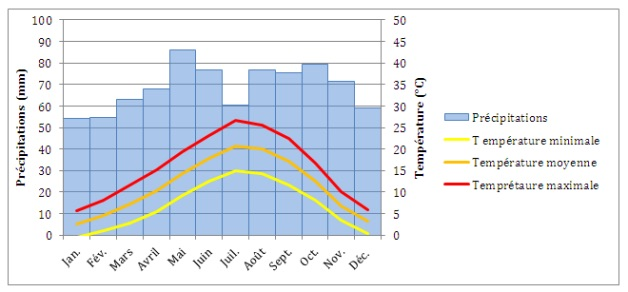
\includegraphics[width=\linewidth]{graphics/DiagrammeThil.jpg}
				\end{center}
			\end{wrapfigure}

			We tested DeCAF in 35 case studies taken from the DUD-E database, to evaluate its power to discriminate between active and inactive molecules.
			We used DeCAF as a classifier and compared it to the SEA (Similarity Ensemble Approach) algorithm \cite{keiser2007relating}.
			To compare sets of ligands, we adapted the approach used in SEA, replacing Tc by DCAF.
			We prepared datasets as shown in the left diagram.
			Then, we tested both classifiers calculating ROC AUC values for every target (below).

			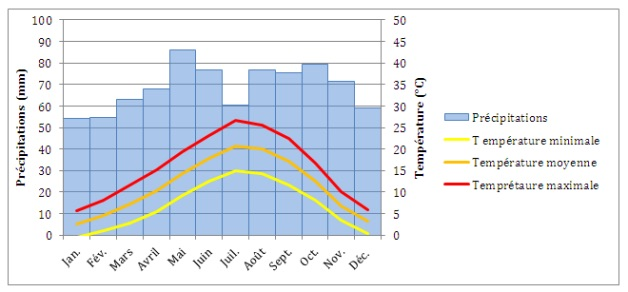
\includegraphics[width=0.95\linewidth]{graphics/DiagrammeThil.jpg}
		}
		\headerbox{6. Conclusions}{name=conclusion,column=1,below=sea,span=2,above=bottom}{
			% DeCAF is a chemoinformatical tool that can be helpful in ligand-based drug design.
			% It provides a comprehensive molecule description and a fast algorithms for comparing and aligning multiple ligands.
			Pour le problème… nous avons proposé une solution basée sur… et nous avons montré
			\begin{boenumerate}\compresslist
				\item qu'elle est conforme aux normes de l'entreprise (fonctionnalisés, intégration avec les autres applications et qualité de code),
				\item que les performances obtenues sont largement suffisante pour supporter les applications actuelles et les évolutions prévues
				\item que les utilisateurs sont satisfaits (étude d'usage non inclue dans ce poster)
			\end{boenumerate}

			La solution proposée est en production depuis deux mois.
			% It can be also used in other [procedures], such as database screening or drug repositioning.
			% DeCAF is written in Python and freely available at \textbf{\color{darkgreen}http://bitbucket.org/marta-sd/decaf}.
		}
		\headerbox{7. References}{name=references,column=0,span=1,below=mcs,above=bottom}{
			%\small % Reduce the font size in this block
			\renewcommand{\section}[2]{\vskip 0.05em} % Get rid of the default "References" section title
			%\nocite{*} % Insert publications even if they are not cited in the poster
			\bibliographystyle{unsrt}
			\bibliography{rapportPFE} % Use sample.bib as the bibliography file
		}
	\end{poster}
\end{document}